\section{Gotta Go Fast!}
\label{GottaGoFast}
In this section we will run benchmarks to test our autotunner. There was an
existing autotunner for Futhark \cite{oldtune}, which was based on OpenTunner
\cite{opentunner}. The existing autotunner uses hill-climbing techniques, on a
filtered set of possible threshold settings, as opposed to ours, that perform
an exhaustive search. We will be comparing the existing autotunner to ours,
with executing without tuning being the baseline. We benchmark on four programs \cite{ppopp}. When autotuning we use Futharks build in benchmarking tool \texttt{futhark bench}\footnote{The documentation for \texttt{futhark bench} can be found here \url{https://futhark.readthedocs.io/en/latest/man/futhark-bench.html}}. \texttt{futhark bench} defaults to executing each dataset ten times and gives back the average. Along with those ten times, we execute the \texttt{bench} five times in creating our graphs, this ends up in fifty runs for each dataset, we do this to avoid deviation in the results.  

We have benchmarked on a Ubuntu 18.04 system with a \textbf{GeForce GTX 1050 4 GB} gpu, and with the NVIDIA driver version: 396.54.  

\paragraph{nn, backprop and matmul}
For the \texttt{nn}, \texttt{backprop}, and \texttt{matmul} program we have two datasets for each \texttt{(D)}, \texttt{(H1, H2)}, and \texttt{(F1, F2)} respectively, with corresponding training sets. 
\begin{figure}[h]
	\centering
	\subfloat[The result for autotuning the \textit{nn} program, with no tuning being the baseline.]{
	\centering
	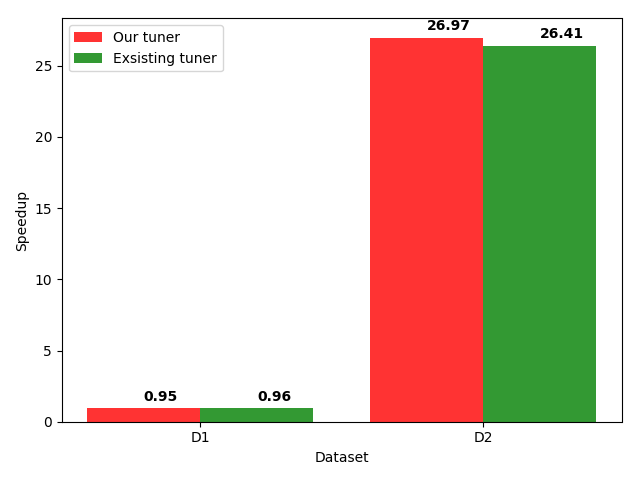
\includegraphics[width=.45\textwidth]{../benchmarks/nn.png}
	\label{nn}}
	\hspace{5mm}
	\subfloat[The result for autotuning the \textit{backprop} program, with no tuning being the baseline.]{
	\centering
	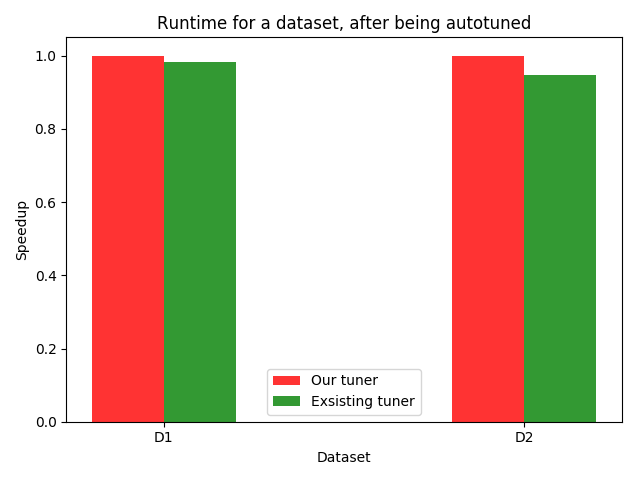
\includegraphics[width=.45\textwidth]{../benchmarks/backprop.png}
	\label{backprop}}
	\hspace{5mm}
	\subfloat[The result for autotuning the \textit{matmul} program, with no tuning being the baseline.]{
	\centering
	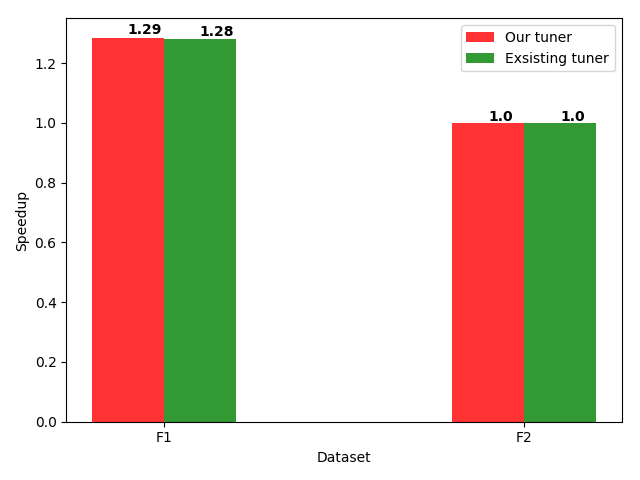
\includegraphics[width=.45\textwidth]{../benchmarks/matmul.png}
	\label{matmul}}
	\caption{Benchmark for \texttt{nn}, \texttt{backprod}, and \texttt{matmul}}
	\label{NNandBackprop}
\end{figure}
In Figure \ref{nn} we clearly see that our autotuner produced a set of thresholds that improved \texttt{D} massively. 

In Figure \ref{backprop} we see that the neither dataset was affected by our tuning, this would lead us to believe that the default values for the thresholds is a good choice for this program with the datasets \texttt{H1, H2}.

And finally in Figure \ref{matmul} we see that matrix multiplication experience an approximately 30\% speedup for \texttt{F1} but is equal in \texttt{F2}. Matrix multiplication runs well on large threshold parameters, which explain the relatively small speedup, since the thresholds, by default, are quite large.

\paragraph{LocVolCalib}
There are three datasets for the \texttt{LocVolCalib} program, \textit{small,
medium} and \textit{large}, as well as a training set for each size.

In Figure \ref{LocVolCalib-SmallMediumLarge}, we have autotunned for the
\textit{small}, \textit{medium} and \textit{Large} datasets, and executed the program on all
three. We plot the speedup, or slow down, compared to executing without
tuning\footnote{Where the default value for thresholds is $2^{15}$, which is
quite high, meaning that it will favor large datasets}.
\begin{figure}[h]
	\centering
	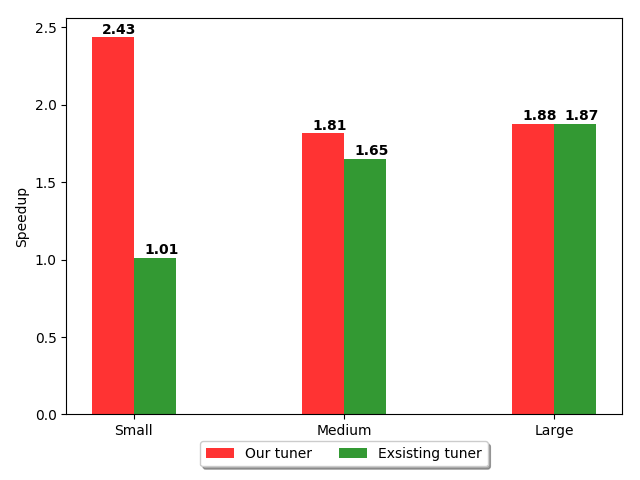
\includegraphics[width=.7\textwidth]{../benchmarks/LocVolCalib.png}
  \caption{The result for autotuning the \textit{LocVolCalib} program, with no tuning being the baseline.}
	\label{LocVolCalib-SmallMediumLarge}
\end{figure}
In Figure \ref{LocVolCalib-SmallMediumLarge} we see that on all datasets the
threshold values our auto-tuner produced improved the performance of the
program. It's also clear that our auto-tuner found a set of values that made
the program perform better on \textit{small} and \textit{medium} than the
existing auto-tuner. The one problem, which cannot be seen in this graph is the
time it takes for each of the auto-tuners to tune the program. For the existing
auto-tuner it took around 17 minutes, whereas for our auto-tuner it took a
little under 23 hours, which is obviously far to slow to be of use in almost
all cases. 

Since \texttt{LocVolCalib} is so slow when autotuning, we also tested how well
it performed when trained on only a subset of datasets, and the result of this
can be seen in Figure \ref{LocVolCalibAll}. The motivation behind this
experiment was that the number of possible combinations dropped drastically as
the number of datasets were reduced. So if near equal results could be gotten
with less datasets the tuning time would be more bearable.

\begin{figure}[H]
	\centering
	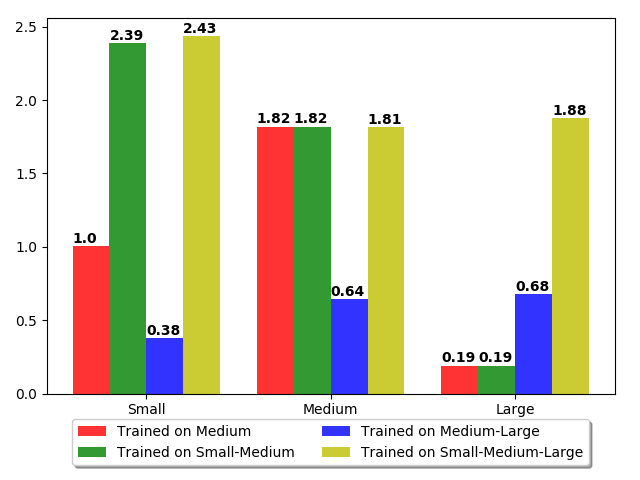
\includegraphics[width=.7\textwidth]{../benchmarks/LocVolCalibAll.png}
  \caption{The result for autotuning the \textit{LocVolCalib} program, for different combinations of datasets, with no tuning being the baseline.}
	\label{LocVolCalibAll}
\end{figure}
